\subsection{Kalibrasi Kamera}

Kamera Leopard yang digunakan pada kendaraan memiliki lensa bidang pandang lebar sebesar 120\textdegree\ sehingga memerlukan kalibrasi untuk menghilangkan distorsi dan membangun model proyeksi.
Kalibrasi dilakukan menggunakan metode \emph{Omnidirectional Camera Calibration} Scaramuzza~\parencite{Scaramuzza2006ICVS} dengan pola papan catur pada beberapa orientasi berbeda.

\begin{figure}[H]
    \centering
    \begin{subfigure}[b]{0.48\textwidth}
        \centering
        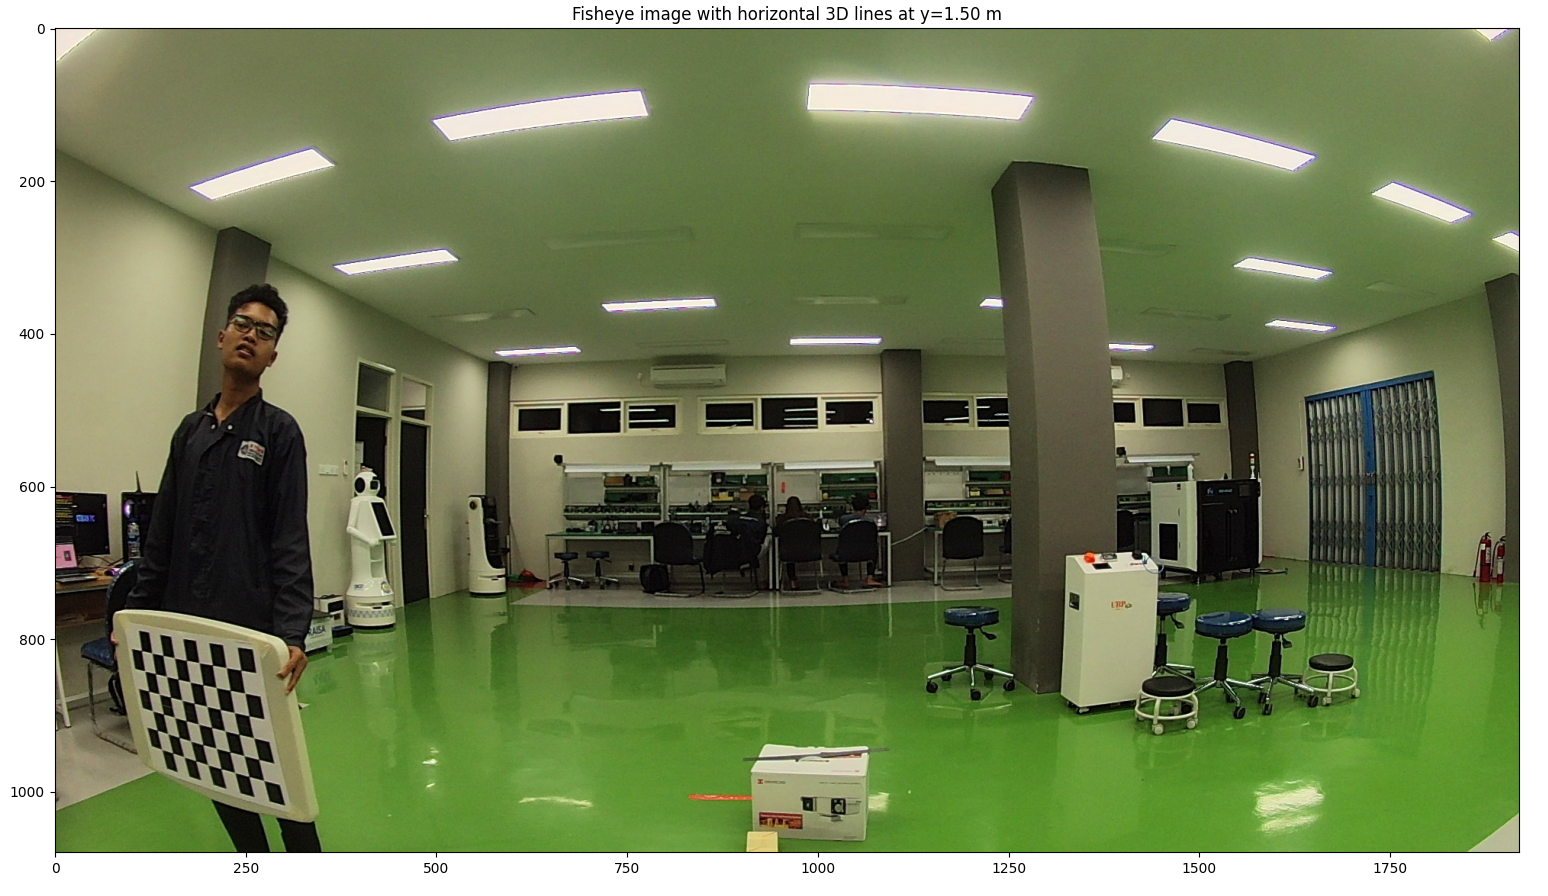
\includegraphics[width=\textwidth]{gambar/camera_before.png}
        \caption{Citra asli dengan distorsi lensa}
        \label{fig:camera_before}
    \end{subfigure}
    \hfill
    \begin{subfigure}[b]{0.48\textwidth}
        \centering
        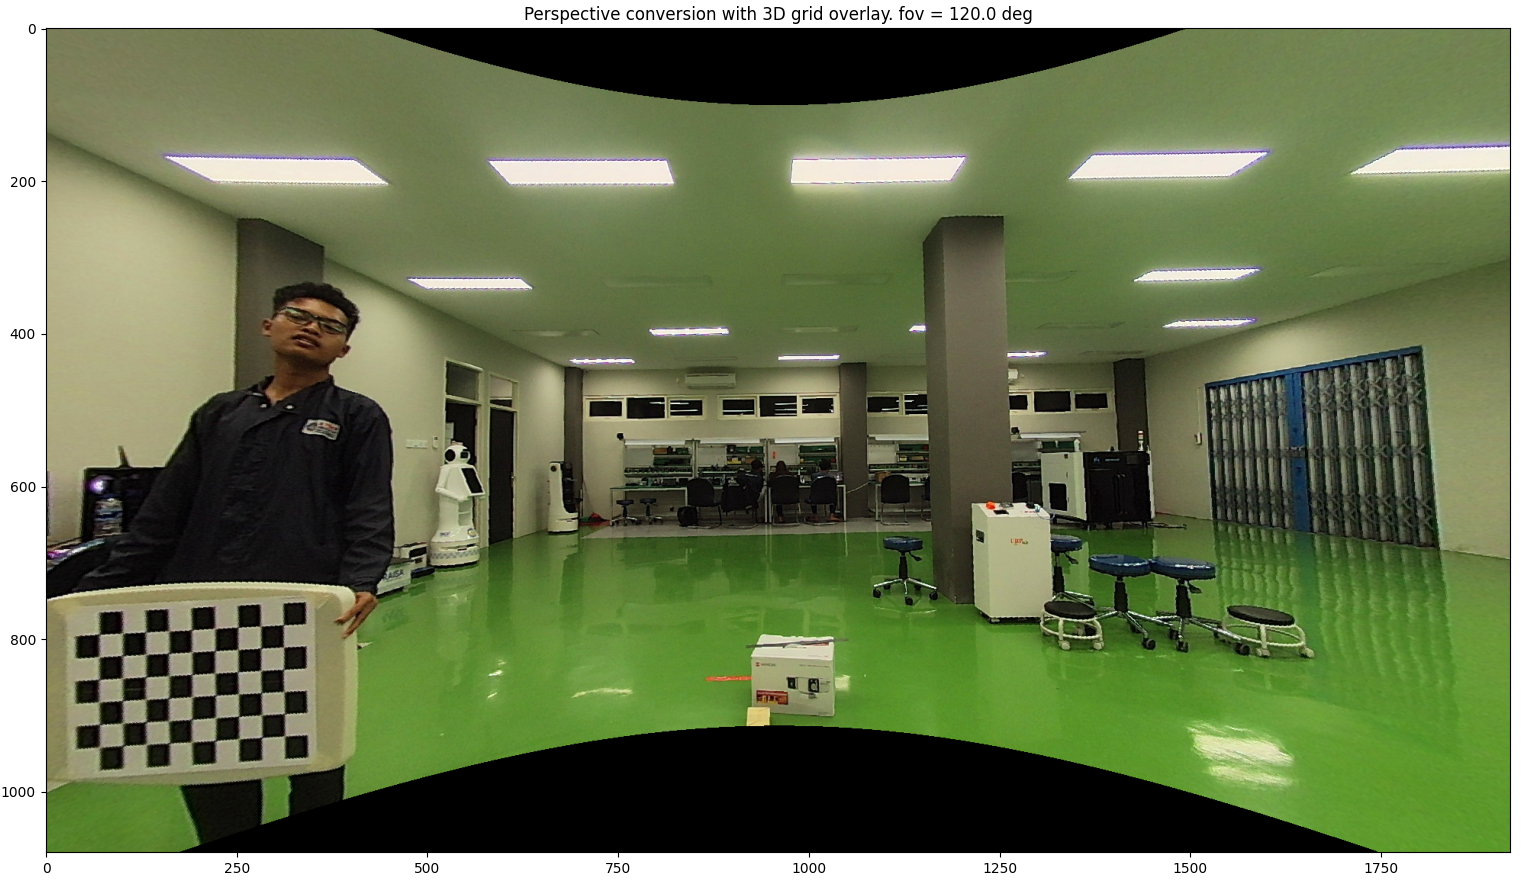
\includegraphics[width=\textwidth]{gambar/camera_rectified.png}
        \caption{Citra setelah kalibrasi dan \emph{rectification}}
        \label{fig:camera_after}
    \end{subfigure}
    
    \medskip
    
    \begin{subfigure}[b]{0.8\textwidth}
        \centering
        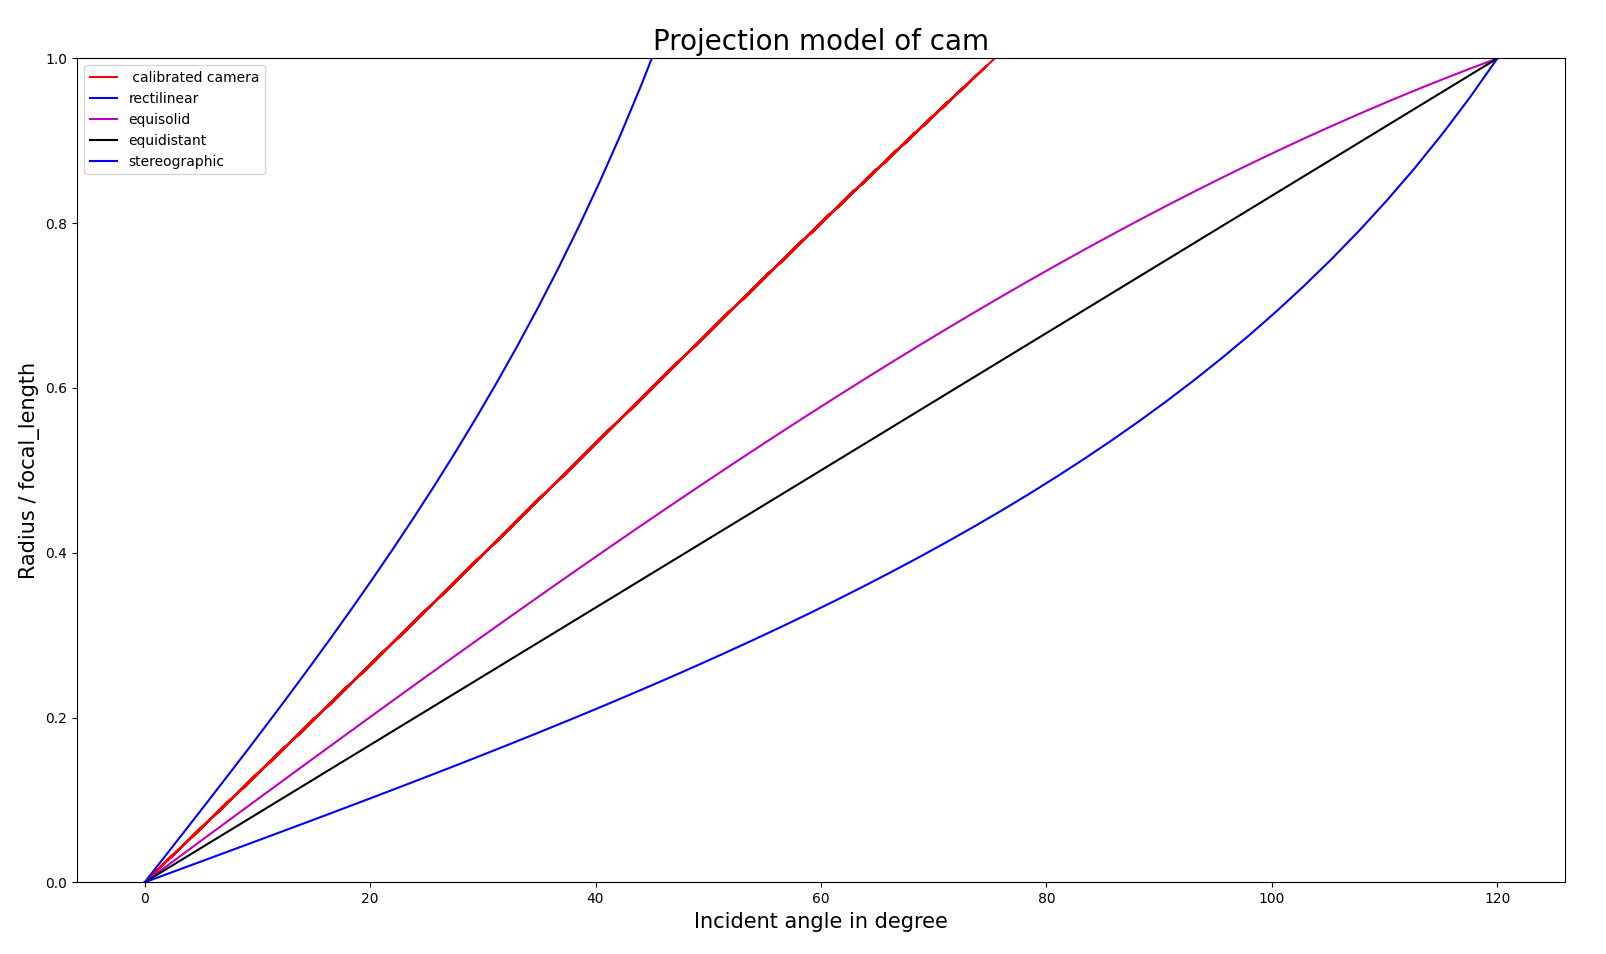
\includegraphics[width=\textwidth]{gambar/projection_model_cam.png}
        \caption{Model proyeksi kamera hasil kalibrasi Scaramuzza.}
        \label{fig:projection_model}
    \end{subfigure}
    \caption{Hasil kalibrasi kamera menggunakan metode Scaramuzza.}
    \label{fig:camera_calibration}
\end{figure}

Dapat dilihat pada gambar diatas bahwa citra yang awalnya mengalami distorsi lensa (Gambar \ref{fig:camera_before}) telah berhasil dikoreksi menjadi citra yang lebih geometris (Gambar \ref{fig:camera_after}) sesuai dengan dunia nyata.
Kemudian didapatkan model proyeksi kamera berupa parameter intrinsik dan koefisien polinomial yang memetakan koordinat piksel pada citra ke koordinat 3D di dunia nyata, yang ditampilkan pada Gambar \ref{fig:projection_model}.
Model proyeksi ini digunakan untuk membangun matriks transformasi yang mampu memetakan piksel citra dari koordinat 2D menjadi koordinat 3D, sehingga memungkinkan konversi dari citra kamera ke tampilan tampak atas (BEV).

\begin{figure}[H]
    \centering
    \begin{subfigure}[b]{0.8\textwidth}
        \centering
        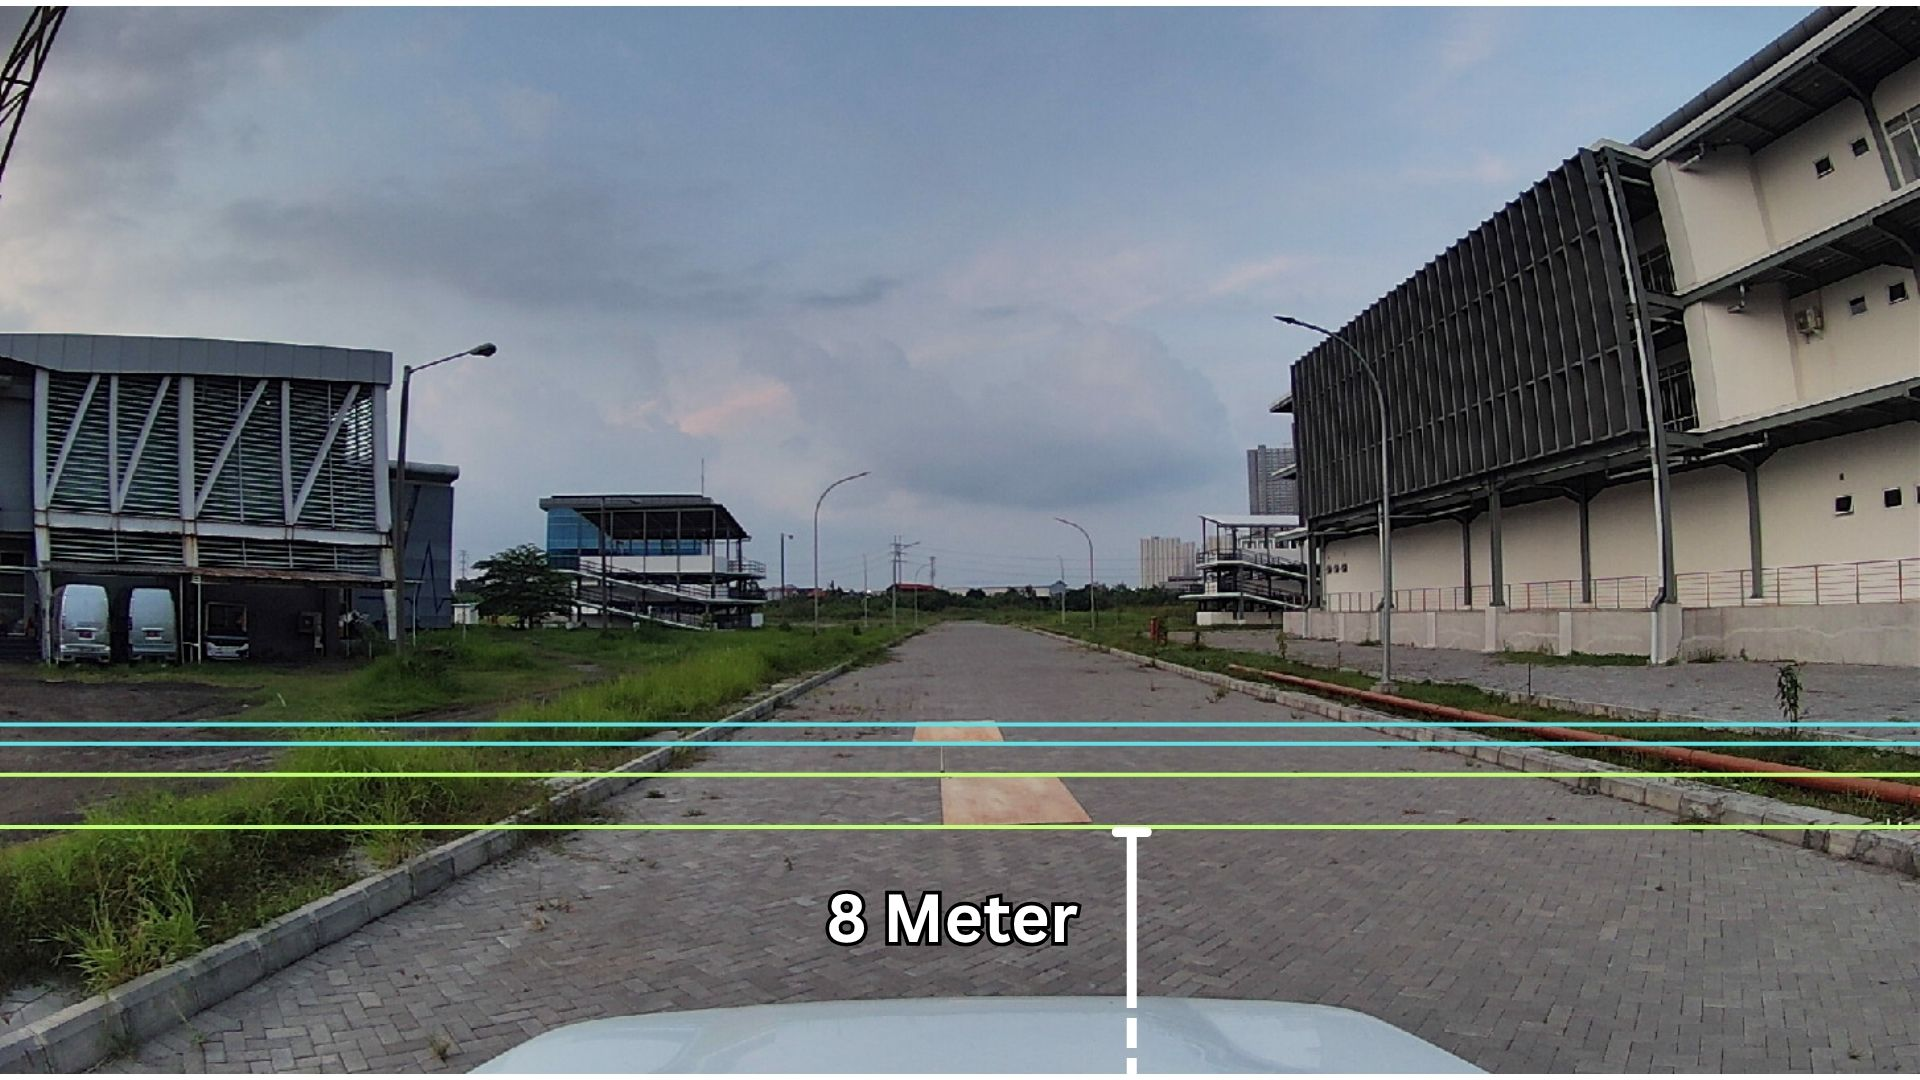
\includegraphics[width=\textwidth]{gambar/kalibrasi_foto.jpg}
        \caption{Tampilan kamera tampak depan ketika validasi transformasi BEV}
        \label{fig:kalibrasi_1}
    \end{subfigure}
    \hfill
    \begin{subfigure}[b]{0.8\textwidth}
        \centering
        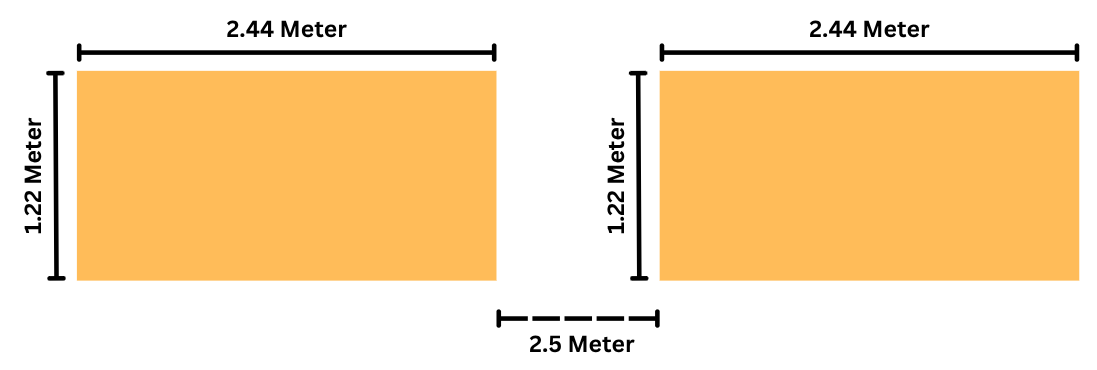
\includegraphics[width=\textwidth]{gambar/kalibrasi_plan.png}
        \caption{Dimensi dan penempatan papan kalibrasi untuk validasi transformasi BEV}
        \label{fig:kalibrasi_2}
    \end{subfigure}
    \caption{Validasi transformasi BEV menggunakan papan kalibrasi.}
    \label{fig:proses_bev_calibration}
\end{figure}

Validasi transformasi BEV dilakukan dengan menggunakan papan kalibrasi yang ditempatkan sejauh 8 meter di depan kendaraan yang diukur dari pusat kamera.
Penempatan papan yang ditunjukkan pada Gambar \ref{fig:kalibrasi_1} memungkinkan untuk melakukan pengukuran jarak secara akurat menggunakan pita ukur.
Terdapat 2 papan kalibrasi yang diletakkan secara sejajar dengan jarak antar papan sebesar 2,5 meter dan memiliki panjang 2,44 meter dan lebar 1,22 meter yang ditunjukkan pada Gambar \ref{fig:kalibrasi_2}.
Dari data yang diperoleh, citra ketika proses kalibrasi ditransformasikan menggunakan matriks transformasi yang diperoleh dari kalibrasi Scaramuzza, sehingga menghasilkan citra tampak atas (BEV) kalibrasi yang menunjukkan posisi papan kalibrasi sesuai dengan jarak sebenarnya yang ditunjukkan pada Gambar \ref{fig:bev_validation}.
Hasil validasi menunjukkan bahwa transformasi BEV yang diperoleh dari kalibrasi Scaramuzza mampu memetakan piksel citra ke koordinat dunia nyata dengan akurasi yang dapat diterima, sehingga dapat digunakan untuk konversi mask segmentasi visual ke representasi \emph{point cloud} yang akurat untuk perencanaan navigasi.

\begin{figure}[H]
    \centering
    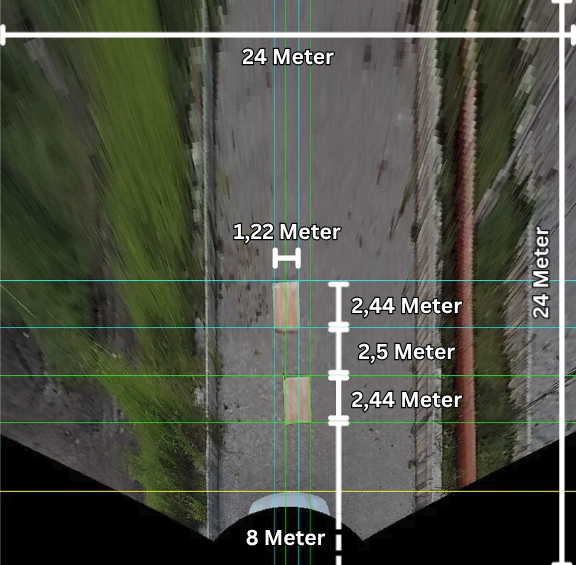
\includegraphics[width=0.8\textwidth]{gambar/hasil_kalibrasi_bev_gambar.png}
    \caption{Hasil validasi transformasi BEV menggunakan papan kalibrasi}
    \label{fig:bev_validation}
\end{figure}

\subsection{Pelatihan Model Segmentasi}

Model InternImage dengan \emph{backbone} DCNv3~\parencite{wang2023internimage} dipilih sebagai arsitektur segmentasi semantik.
Model ini dipralatih pada dataset Mapillary Vistas yang berskala global sehingga telah memiliki kemampuan dasar dalam mengenali berbagai tipe jalan dan lingkungan perkotaan.
Selanjutnya dilakukan \emph{fine-tuning} pada dataset lokal kampus ITS agar model dapat beradaptasi dengan karakteristik visual jalan di lingkungan pengujian.

Dataset lokal terdiri dari 2200 citra yang dibagi menjadi 80\% untuk pelatihan dan 20\% untuk validasi.
Citra diambil menggunakan kamera depan kendaraan Omoda E5 pada berbagai kondisi pencahayaan yang terdiri dari siang terik, mendung, dan hujan.

Pelabelan dilakukan secara manual menggunakan perangkat lunak LabelMe dan RoboFlow, di mana setiap piksel pada citra diberi label \emph{road} (jalan yang dapat dilalui) atau \emph{background} (non-jalan).
Hasil pelabelan disimpan dalam format JSON dan dikonversi menjadi mask biner dua kelas.
Proses pelabelan diilustrasikan pada Gambar~\ref{fig:labelme}, sedangkan contoh mask biner yang dihasilkan ditunjukkan pada Gambar~\ref{fig:mask_labelme}.

\begin{figure}[H]
    \centering
    \begin{subfigure}[b]{0.75\textwidth}
        \centering
        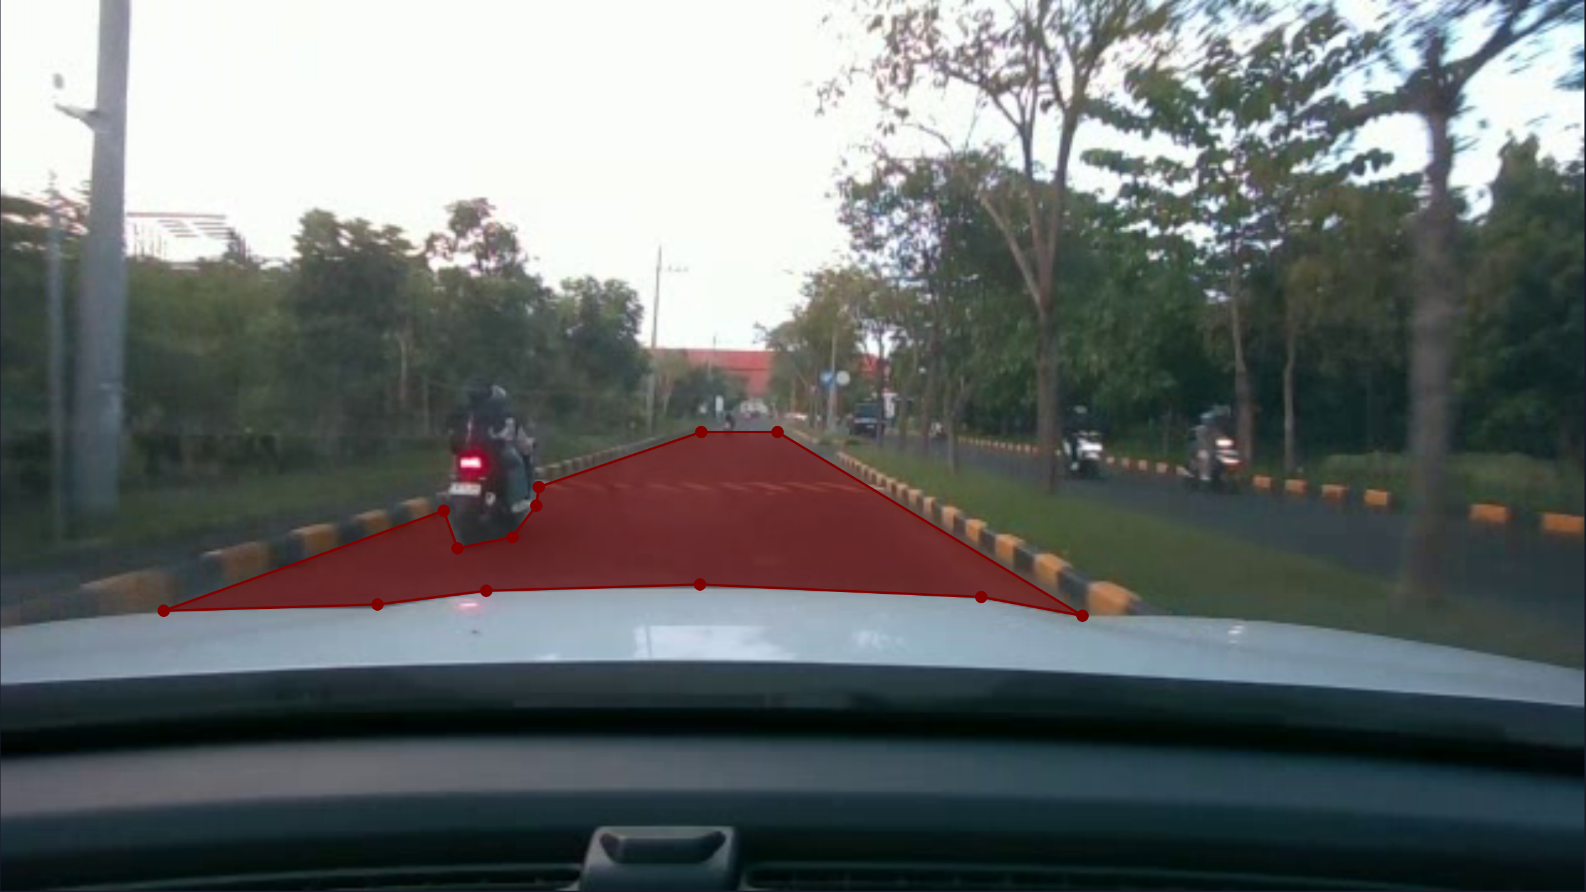
\includegraphics[width=\textwidth]{gambar/labelme.png}
        \caption{Proses pelabelan dengan LabelMe}
        \label{fig:labelme}
    \end{subfigure}
    \hfill
    \begin{subfigure}[b]{0.8\textwidth}
        \centering
        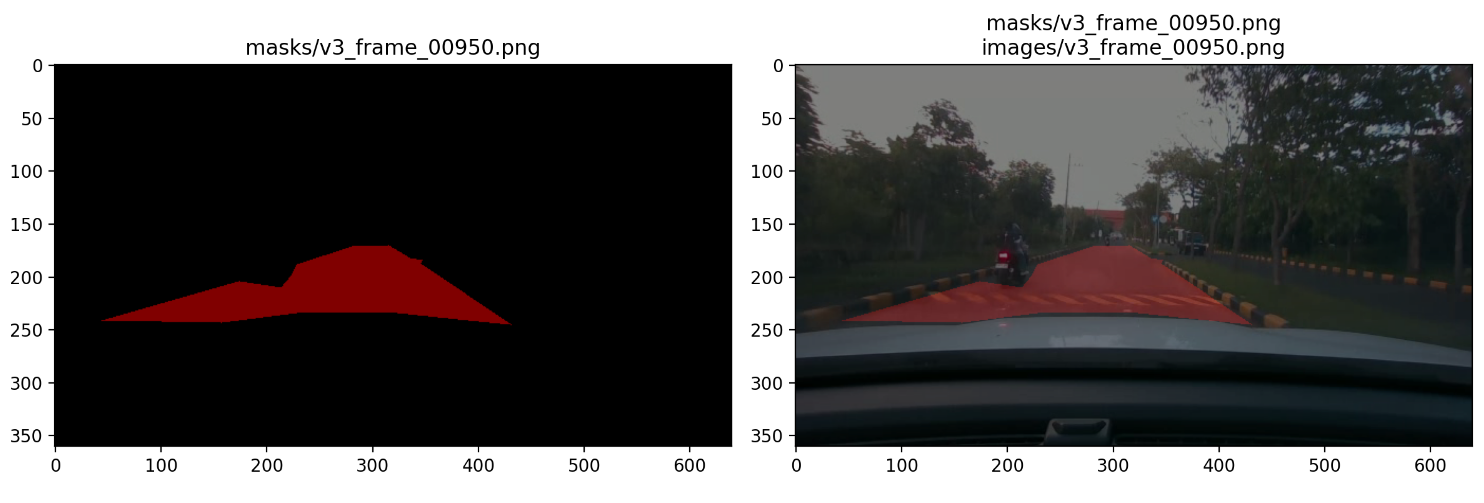
\includegraphics[width=\textwidth]{gambar/mask_labelme.png}
        \caption{Contoh masker biner dua kelas}
        \label{fig:mask_labelme}
    \end{subfigure}
    \caption{Proses pelabelan dataset segmentasi visual.}
    \label{fig:pelabelan}
\end{figure}

Model dilatih menggunakan kombinasi \emph{Cross-Entropy Loss} dan \emph{Dice Loss} dengan optimizer AdamW.
\emph{Learning rate} diatur sebesar $6\times10^{-6}$ untuk \emph{backbone} dan $6\times10^{-5}$ untuk \emph{classification head}, dengan \emph{scheduler Cosine Annealing} dan 5 epoch \emph{warmup}.
Ukuran \emph{batch} yang digunakan adalah 4 citra dengan resolusi masukan $512\times512$ piksel.
Pelatihan dilakukan pada GPU NVIDIA RTX 4060 selama 50 epoch.

\subsection{Optimasi Inferensi dengan TensorRT}

Model hasil training PyTorch (.pth) dikonversi ke format ONNX dan selanjutnya dioptimasi menjadi \emph{engine} TensorRT menggunakan presisi FP16.
Alur konversi dari model PyTorch ke \emph{engine} TensorRT diilustrasikan pada Gambar~\ref{fig:tensorrt_workflow}.

\begin{figure}[H]
    \centering
    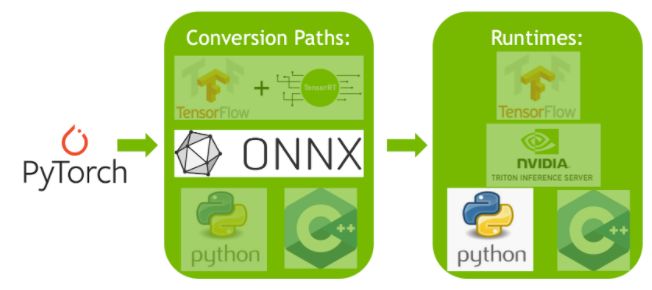
\includegraphics[width=0.8\textwidth]{gambar/tensorrt_workflow.png}
    \caption{Alur konversi model PyTorch ke \emph{engine} TensorRT melalui format ONNX \parencite{NVIDIATensorRT}.}
    \label{fig:tensorrt_workflow}
\end{figure}

Teknik \emph{layer fusion} menggabungkan beberapa \emph{layer} berurutan menjadi satu operasi GPU untuk mengurangi \emph{overhead} memori.
Target laju inferensi adalah di atas 15 FPS pada GPU NVIDIA RTX 4060 agar memenuhi kebutuhan navigasi \emph{real-time} pada kecepatan rendah.

\subsection{Konversi Mask ke \emph{Point Cloud}}

Masker biner hasil segmentasi visual kemudian dikonversi dengan matriks transformasi BEV yang diperoleh dari kalibrasi kamera untuk menghasilkan masker biner BEV seperti yang ditunjukkan pada Gambar~\ref{fig:mask_bev}.

\begin{figure}[H]
    \centering
    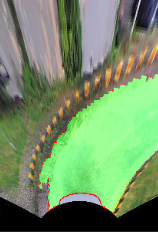
\includegraphics[width=0.4\textwidth]{gambar/masker_bev.png}
    \caption{Masker biner hasil transformasi BEV}
    \label{fig:mask_bev}
\end{figure}

Dari hasil masker biner BEV tersebut, dapat dilakukan proses morfologi untuk menghilangkan \emph{noise} dan mengisi lubang pada masker, sehingga menghasilkan masker yang lebih bersih dan kontinu.
Kemudian masker tersebut dilakukan proses deteksi garis tepi untuk menemukan batas area jalan yang dapat dilalui.
Garis tepi yang terdeteksi perlu melalui proses \emph{masking} untuk menghilangkan garis yang tidak relevan seperti garis tepi mobil atau batas frame citra yang tidak termasuk area jalan.
Setelah garis tepi yang relevan berhasil diekstraksi, titik-titik pada garis tepi tersebut diekstraksi sebagai representasi \emph{point cloud} yang merepresentasikan area jalan yang dapat dilalui.